\subsection{Diferencias entre BCIs SSVEP y NextMind}

A pesar de que NextMind es bastante reservado sobre el funcionamiento interno de su dispositivo, hay varios aspectos clave que lo diferencian de los BCIs SSVEP tradicionales.

\subsubsection{Arquitectura}

NextMind emplea una arquitectura única que se centra en el lóbulo occipital, una región cerebral responsable de la interpretación de la información visual. A diferencia de otros BCIs que requieren un casco completo para cubrir múltiples regiones cerebrales, NextMind es un dispositivo compacto y liviano que se coloca en la parte posterior de la cabeza, proporcionando una mayor comodidad para el usuario.

\subsubsection{Sistema Híbrido: Inteligencia Artificial}

Una de las características más notables de NextMind es su uso de inteligencia artificial para mejorar la precisión y la eficiencia del dispositivo. NextMind implementa una red neuronal que el usuario debe entrenar inicialmente para que el dispositivo pueda ajustarse mejor a las señales cerebrales específicas del usuario. Este enfoque híbrido facilita una adaptación más personalizada y eficiente a las respuestas cerebrales individuales.

\subsubsection{Patrón de Estímulo}

NextMind emplea un patrón de estímulo novedoso para potenciar la captación de las respuestas visuales. En lugar de los patrones convencionales utilizados en los BCIs SSVEP, NextMind utiliza una malla de puntos, donde cada ``neurotag'' parpadea a una frecuencia específica. Esta innovadora forma de estimulación visual puede ayudar a mejorar la detección y el seguimiento de los estímulos visuales por parte del dispositivo.



Un NeuroTag generalmente consiste en un patrón visual o un objeto en una interfaz gráfica que está diseñado para provocar una respuesta neural específica cuando el usuario lo observa. Estas respuestas neuronales pueden ser registradas y decodificadas por la BCI de NextMind, lo que permite al sistema inferir la intención del usuario a través del monitoreo de las reacciones cerebrales a estos neurotags (véase en la figura \ref{figure:nextmind-neurotag})

\begin{figure}[!htb]
   \centering
    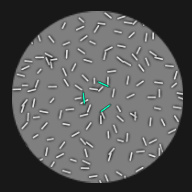
\includegraphics[width=0.4\linewidth]{figures/Neurotag.png}
   \caption{Neurotag de NextMind}
   \label{figure:nextmind-neurotag}
\end{figure}
